\clearpage
\subsection{Assembly} % (fold)
\label{sub:assembly}

The next level of abstraction up from machine code is called \textbf{Assembly}, or \textbf{Assembler Code}. Here the numeric machine code instructions are given symbolic names that are, to some degree, more understandable for humans. The code \texttt{0000 0011} may be given the symbolic name \texttt{add}, for example.

Programs written in this language cannot be executed directly by the computer, it isn't machine code. Assembler code is converted to machine code by a program called an \textbf{Assembler}. This program reads the instructions from the assembler code and outputs machine code. So, for example, anywhere it encounters \texttt{add} in the code it can output \texttt{0000 0011}.

\begin{figure}[h]
   \centering
   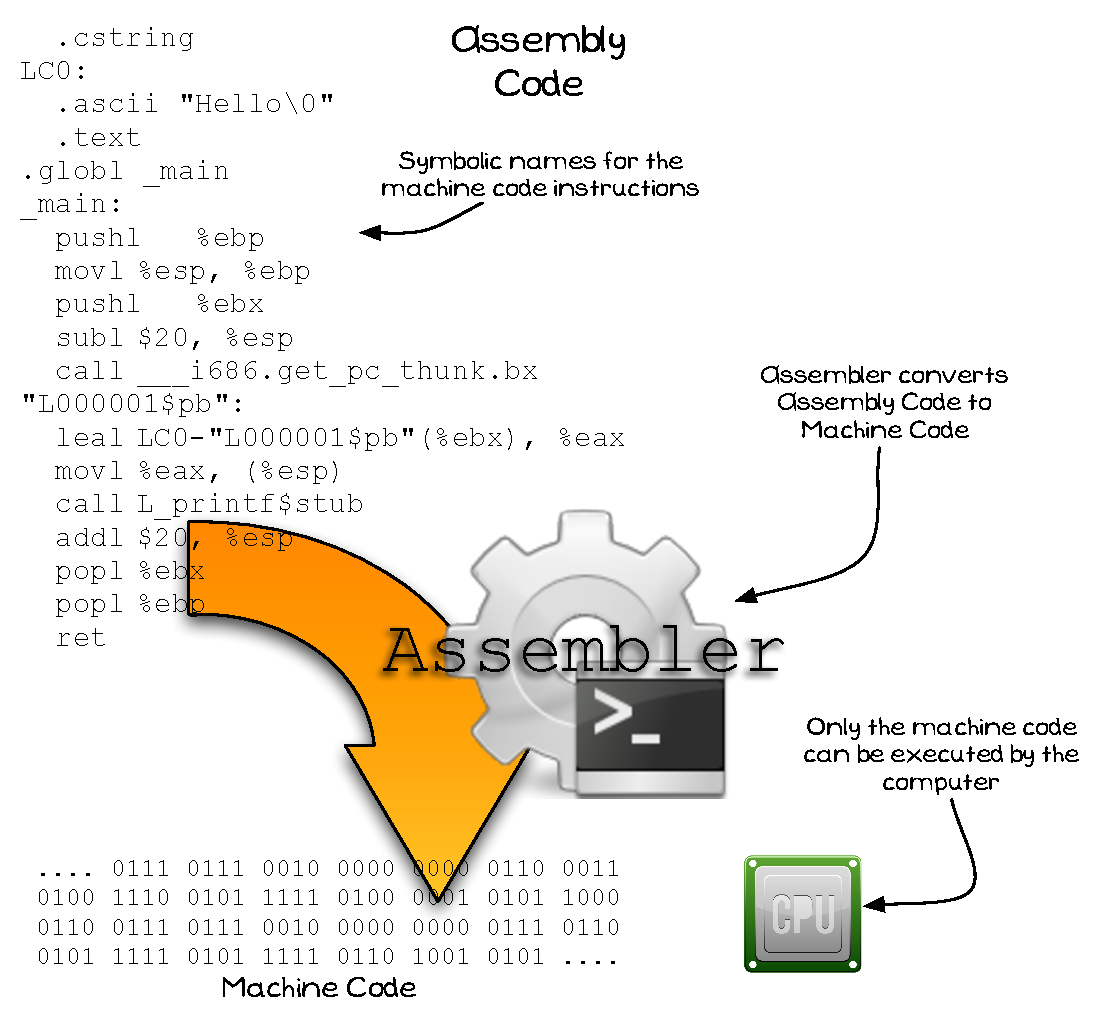
\includegraphics[width=0.8\textwidth]{./topics/programs-and-compilers/diagrams/Assembly} 
   \caption{The computer responds to machine code instructions}
   \label{fig:assembly}
\end{figure}

\mynote{
\begin{itemize}
  \item As with \nameref{sub:machine_code}, Assembly is liked to individual CPUs.
  \item Assembly is very close to Machine Code, its machine code with symbolic names for the instructions.
\end{itemize}
}

\clearpage
\subsubsection{Programming in Assembly} % (fold)
\label{ssub:programming_in_assembly}

The code in Listing \vref{asmcode} shows an example of some assembler code. This is the assembler code that was used to generate the machine code from Listing \ref{lst:machine code}. The machine code was 13,344 bytes in size, where the same program in assembler code is only 658 bytes. The assembler reads these 658 bytes, combines it with instructions from program libraries, and outputs machine code. 
\lstset{language=[x86masm]{assembler}}

\begin{lstlisting}[caption={Assembler Sample},label={asmcode}]
  .cstring
LC0:
  .ascii "Hello\0"
  .text
.globl _main
_main:
  pushl	%ebp
  movl	%esp, %ebp
  pushl	%ebx
  subl	$20, %esp
  call	___i686.get_pc_thunk.bx 
"L000001$pb":
  leal	LC0-"L000001$pb"(%ebx), %eax
  movl	%eax, (%esp)
  call	L_printf$stub
  addl	$20, %esp
  popl	%ebx
  popl	%ebp
  ret
\end{lstlisting}

From a programmer's perspective, assembler code is much easier to work with than machine code, though there are still issues with the use of assembler code. Firstly Assembly is bound to the instruction set of the CPU that you are targeting, meaning that if you want to support other kinds of CPU you will need to rewrite the program. The other main issue with assembler code is that while it is more understandable, you are still working with the primitive instructions of the CPU. Working at this level takes considerable effort to write even simple programs.

Assembly languages were first developed in the 1950s, and were known as a \textbf{Second Generation}\footnote{First Generation being Machine Code.} programming languages. This step forward did make programming easier, but the tools have advanced since then and now we can work at an even higher level of abstraction.

% subsubsection programming_in_assembly (end)

% subsection assembly (end)